\documentclass{article}

\title{EE 371 Autumn 2016 - Lab 1}
\date{\today}
\author{William Li, Jun Park, Dawn Liang}

% general document formatting
\usepackage[margin=1in]{geometry}
\usepackage[document]{ragged2e}
\usepackage{times}

\usepackage{titlesec}
\titleformat{\section}{\Large\bfseries}{\thesection}{0.5em}{\uppercase}

% formatting for code & floats
\usepackage{listings}
\usepackage{color}
\usepackage{graphicx}
\usepackage{float}
\usepackage{wrapfig}

\definecolor{dkgreen}{rgb}{0,0.6,0}
\definecolor{gray}{rgb}{0.5,0.5,0.5}
\definecolor{mauve}{rgb}{0.58,0,0.82}

\lstset{frame=tb,
  language=Verilog,
  aboveskip=3mm,
  belowskip=3mm,
  showstringspaces=false,
  columns=flexible,
  basicstyle={\small\ttfamily},
  numbers=none,
  numberstyle=\tiny\color{gray},
  keywordstyle=\color{blue},
  commentstyle=\color{dkgreen},
  stringstyle=\color{mauve},
  breaklines=true,
  breakatwhitespace=true,
  tabsize=3
}

\begin{document}

\newcommand{\namesigdate}[2][5cm]{
  \begin{tabular}{@{}p{#1}@{}}
    #2 \\[2\normalbaselineskip] \hrule \\[0pt]
    {\small \textit{Signature}} \\[2\normalbaselineskip] \hrule \\[0pt]
    {\small \textit{Date}}
  \end{tabular}
}

\pagenumbering{gobble}
\maketitle
\newpage

\paragraph{} We certify that the work in this report is our own, and that any work that is not ours is cited.

\paragraph{} \noindent \namesigdate{William Li} \hfill \namesigdate{Dawn Liang} \hfill \namesigdate{Jun Park}
\newpage

\tableofcontents
\newpage

\pagenumbering{arabic}

\section{Abstract}
\paragraph{} This lab focuses on introducing us to the tools and methods of digital design. We were introduced to the four levels of abstraction in modeling and implementation with Verilog on the Altera DE1-SoC board. Then, we familiarised ourselves with the tools involved in designing and testing hardware applications with Quartus. Additionally, we were introduced to the general design process for hardware and software and applications.

\section{Introduction}
\paragraph{} This lab focuses on designing and building VHDL (Verilog Hardware Description Language) programs. First, we built four different types of counters using different modeling techniques: a 4-bit ripple up counter using gate modeling, a 4-bit synchronous up counter using both dataflow model and schematic entry, and a 4-bit synchronous Johnson up counter using the behavioural model. In the process of building and testing these counters, we were introduced to Icarus Verilog (iVerilog) and GTKWave software, for compiling our designs and simulating waveforms. We then loaded our designs onto an Altera Cyclone V FPGA, where we verified their functionality on hardware. Then we utilised Signal Tap II, a logic analyzer for probing designs in hardware. Finally, we were briefly introduced to the C programming language. We learned the basics of a C program in the CodeBlocks IDE by compiling a provided C project, and then we built a simple C car price calculator program that asks for relevant input data and outputs an approximate list price for a brand new vehicle.



\section{Discussion}
  \subsection{Design}
	  \subsubsection{Design Specification}
	  	\paragraph{} We built four different types of counters: a ripple-up counter, two synchronous up counters, and a Johnson counter, all of which counted on every positive clock edge. All the counters we built had active low reset. The first three counters were directly written in SystemVerilog, the fourth counter was designed using Quartus’ schematic entry feature. The ripple-up and synchronous counters counted up in binary, while the Johnson counter counted up by the most significant bit. The listPrice calculator was to take appropriate input data and calculate the estimated price of a new car. The program prompts the user for the manufacturer’s cost, the estimated dealer’s markup, the pretax discount, and the sales tax, and then outputs the estimated list price.

	  	\paragraph{} The list price calculator was to take appropriate input data and calculate the estimated price of a new car. The program prompts the user for the manufacturer's cost, the estimated dealer's markup, the pre-tax discount, and the sales tax, and then calculates and outputs the estimated list price.

	  \subsubsection{Design Procedure}
	  	\paragraph{} In Verilog HDL, we designed and implemented four counters using three different levels of modeling abstraction: structural/gate-level, dataflow, and behavioural. The first three counters were implemented using the D-flipflop provided in the lab spec; the fourth counter was implemented via Quartus' schematic entry feature.
	  	\lstinputlisting[language=Verilog]{../counters/DFlipFlop.v}

		  \begin{wrapfigure}{R}{0.4\textwidth}
		  	\centering
		  	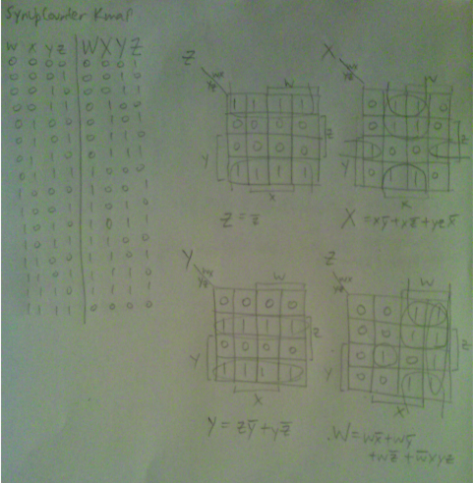
\includegraphics[width=0.4\textwidth]{figures/synch_k_maps.png}
		  	\caption{Truth table \& K-map logic reduction for synchronous counter}
		  	\label{fig:synCounter_kmap}
		  \end{wrapfigure}

		  \paragraph{}The ripple-up counter was implemented at the structural level. The connections between the D-flipflops and outputs were explicitly assigned based on the gate-level diagram. Then, a testbench was written to verify its behaviour using iverilog and gtkwave simulations. The design was then loaded onto the DE1-SoC board through Quartus and probed using Signal Tap II Logic Analyser, to see if its performance on hardware matched expected ideal behaviour in simulation.

		  \paragraph{}The first synchronous up counter was implemented at the dataflow level. We diagrammed the states and generated boolean expressions using truth tables and K-maps, depicted on the right. We then drew the gate-level diagram from those expressions, and wrote Verilog code from that. The testing procedure for this counter was the same as previously described.

		  \paragraph{}The johnson counter was implemented at the behavioural level. All behaviour was described within the verilog code. As the counter was essentially a cycling of inputs, the gate-level diagram was fairly straightforward to draw as well. The testing procedure for this counter was the same as previously described.

		  \paragraph{}The second synchronous up counter was built via schematic entry, a feature of Quartus II. The verilog code was then generated from the schematic, using Quartus' generate HDL feature. We wrote the testbench for this in Quartus, and the rest of the testing procedure was the same as previously described.

	  \subsubsection{System Description}
	  	\paragraph{} The four counters take a clock and an active-low reset as the input, which we wired to the internal 50MHz clock and SW[0] respectively on the DE1-SoC board. For the synchronous counter built with Quartus' schematic entry, we included an active-high 'enable' signal input, which acts as an pause/resume switch, wired to SW[1] on the physical board. All four counters output 4-bits, counting up, outputting to LED's [3:0] on the board

	  	\paragraph{} The list price calculator takes the manufacturer's cost (\$), the estimated markup (\%), the pre-tax discount (\%), and sales tax (\%) as inputs. It then calculates the estimated list price of a vehicle, calculated from those values, and displays it to the user as output.

	  \subsubsection{Software Implementation}
	  	\paragraph{} Each counter module is written in Verilog, and utilises a clock divider and D-FlipFlop submodule. The connections between each submodule were determined by the logic reductions and gate-level designs.

	  	\paragraph{} The listPrice program was written in C, to be executed in the console as a script.

	  \subsubsection{Hardware Implementation}
	  	\paragraph{} The inputs/outputs of the counter modules were directly assigned to pins on the FPGA, using Quartus' pin planner and documentation for our specific device.

  \subsection{Test}
	  \subsubsection{Test Plan}
	  	\paragraph{} The counters were both simulated on our computers using iverilog and gtkwave, to check the software implementation, and then tested on the physical DE1-SoC board, to check the hardware implementation. In simulation, the active-low reset and counting sequence were checked. In the case of the schematic entry counter, the enable signal was also checked. In hardware, the LEDs had to display the four outputs bits and count in the correct sequence; the reset signal should reset to all 0's and restart counting when untriggered. In the case of the schematic entry synchronous counter, the enable signal should pause counting when triggered and resume when untriggered.

	  	\paragraph{} The listPrice calculator was tested with different types of inputs, both expected and invalid inputs. Its output must be verified against external calculations to ensure it is mathematically correct as well.

	  \subsubsection{Test Specification}
	  	\paragraph{} The counters need to be tested such that the reset signal properly resets the output to all 0's, and that the reset signal is active-low. They also need to count in the correct 4-bit sequence, counting each positive clock edge. They should cycle back to their initial state after reaching the maximum state. For the schematic entry synchronous counter, the enable signal should alse pause/resume the counting sequence.

	  	\paragraph{} The listPrice calculator's inputs need to be tested against possible edge cases, such as negative values or invalid inputs like strings. Additionally, expected inputs need to be tested to check that they calculate the correct list price.

	  \subsubsection{Test Cases}
	  	\paragraph{} In simulation, the counters were connected to a clock and reset signal (in the case of the fourth counter, an additional enable signal connected), and the four-bit output bus was monitored. For each counter, the reset was triggered, untriggered, and then the clock ran until the reset was triggered again. The 4-bit outputs were measured to ensure appropriate counting behaviour, counting up at each clock edge and resetting to 0 when triggered.

	  	\paragraph{} On the board, the counters were connected to a switch for reset and four LEDs for outputs (for the fourth counter, an additional switch for enable). The reset was triggered, untriggered, then the clock ran until the reset was triggered again. The 4-bit outputs were monitored on the LEDs, and their behaviour checked to ensure they were counting up at each clock edge and resetting when triggered. In the case of the fourth counter, the enable signal was also checked to see if it paused/resumed counting.

	  	\paragraph{} The listPrice calculator was tested by running the program and checking edge cases. We tested regular, expected inputs, as well as negative value and string inputs, to check handling of unexpected inputs.



\section{Results}

  \paragraph{} In simulation and on the DE1-SoC board, our four counters worked as expected. The waveforms showed that they incremented by 1 bit at each clock edge, cycling back to 0 once the maximum had been reached. They reset to 0 when signaled, showing no signs of metastable behaviour. For the fourth counter, the enable signal properly paused/resumed the counter.

  \paragraph{} On the board, the LEDs corresponding to the 4-bits exhibited appropriate counting behaviour, also cycling back to 0 once the maximum had been reached. When the reset switch was triggered, the LEDs switched off, and resumed counting at 0 when reset was switched off. For the fourth counter, the enable switch properly paused and resumed counting.

  \paragraph{} The designs were probed on the board using Signal Tap II Logic Analyser, and the waveforms generated matched the expected ideal waveforms. There was significantly more noise in the signals immediately after triggers in the Signal Tap data, due to gate delays that occur in real time but not in simulations.

  \paragraph{Comparison of gate-level design to synthesised RTL view} The ripple-up counter we designed is exactly the same as the one Quartus synthesised. The Johnson up counters are also the same, though the Quartus diagram stacks the D-ff's on top of each other for conciseness and simpicity. For the synchronous counter, the diagram we drew was significantly different from the one Quartus synthesized. This is because the logic reduction performed by Quartus is different from the logic reduction we used.

  \paragraph{} The listPrice calculator outputted the correct prices when presented with expected positive numerical inputs. When given invalid inputs, the program also behaves as expected. For negative inputs, the program outputs a mathematically valid but nonsensical result (a negative price). For string inputs, the program throws an error and crashes.



\section{Analysis of Errors}
  \subsection{General Issues}
  \paragraph{} The majority of our issues had to do with difficulty finding documentation, and sometimes outdated documentation, since resources were spread across the class website and not centralised in one place. This was mostly an issue when trying to get Signal Tap II working - figuring out how to set up the environment with regards to the device and the pins. Eventually, with TA help, we found documentation and figured it out.

  \subsection{Failure Modes \& Effects Analysis}
  \paragraph{}We performed failure modes and effects analysis for three counters. Looking at each signal in the gate-level circuit, we considered the effects on the overall circuit if it were 1) stuck at 0 (SA0), or 2) stuck at 1 (SA1).

  \subsubsection{Ripple-up counter}
	\paragraph{} output signal out
	\begin{itemize}
		\item SA0: This means that all the bits Q0 to Q3 are stuck at zero. Therefore even if the clock was operating properly, the counter will never count any positive edges of the clock.
		\item SA1: This means that all the bits Q0 to Q3 are stuck at one. Therefore even if the clock was operating properly, the counter will remain at the binary value 1111, and never wrap back around to zero to count back up. 
	\end{itemize}

	\paragraph{} input signal clk
	\begin{itemize}
		\item SA0: This means that there won’t be any positive clock edges, therefore the counter will stop counting up.
		\item SA1: This means that there won’t be any more positive clock edges beyond this point, therefore the counter will stop counting up. 
	\end{itemize}

	\paragraph{} input signal rst
	\begin{itemize}
		\item SA0: The output will be reset to zero, but it will remain indefinitely at zero.
		\item SA1: The output will be at an unknown state if the rst becomes stuck at 1 from the moment the counter is powered on. If it rst becomes stuck at 1 during operation, the counter will still count up properly, but properly resetting the counter won’t be possible.
	\end{itemize}

	\paragraph{} internal signal Q0
	\begin{itemize}
		\item SA0: The least significant bit of the output will never change from 0 and    the rest of the counter will stop counting up as the cascading clock into the series flipflops get stuck at 1.
		\item SA1: The least significant bit of the output will never change from 1 and the rest of the counter will stop counting up as the cascading clock into the series flipflops get stuck at 0. 
	\end{itemize}

	\paragraph{} internal signal Q1
	\begin{itemize}
		\item SA0: The second least significant bit of the output will never change from 0 and the rest of the counter will stop counting up as the cascading clock into the series flipflops get stuck at 1.
		\item SA1:The second least significant bit of the output will never change from 1 and the rest of the counter will stop counting up as the cascading clock into the series flipflops get stuck at 0. 
	\end{itemize}

	\paragraph{} internal signal Q2
	\begin{itemize}
		\item SA0: The second most significant bit of the output will never change from 0 and the rest of the counter(Q3 bit) will stop counting up as the cascading clock into the series flipflop get stuck at 1. 
		\item SA1: The second most significant bit of the output will never change from 1 and the rest of the counter (Q3 bit) will stop counting up as the cascading clock into the series flipflop get stuck at 0. 
	\end{itemize}

	\paragraph{} internal signal Q3
	\begin{itemize}
		\item SA0: The most significant bit of the output will never change from 0 but otherwise attemps to count up.
		\item SA1:The most significant bit of the output will never change from 1 but otherwise attemps to count up. 
	\end{itemize}

	\paragraph{} internal siganl clkTemp1
	\begin{itemize}
		\item SA0: After the least significant bit  of the output, the counter will stop counting as the cascading clock into the series flipflops get stuck at 0.
		\item SA1: After the least significant bit  of the output, the counter will stop counting as the cascading clock into the series flipflops get stuck at 1. 
	\end{itemize}

	\paragraph{} internal signal clkTemp2
	\begin{itemize}
		\item SA0:  After the second least significant bit  of the output, the counter will stop counting as the  cascading clock into the series flipflops get stuck at 0.
		\item SA1: After the second least significant bit  of the output, the counter will stop counting as the  cascading clock into the series flipflops get stuck at 1. 
	\end{itemize}

	\paragraph{} internal signal clkTemp3
	\begin{itemize}
		\item SA0: After the third least significant bit  of the output, the counter will stop counting as the  cascading clock into the series flipflops get stuck at 0.
		\item SA1: After the third least significant bit  of the output, the counter will stop counting as the  cascading clock into the series flipflops get stuck at 1. 
	\end{itemize}

	\paragraph{} internal signal clkTemp4
	\begin{itemize}
		\item SA0: The most significant bit of the output will be stuck at 0 indefinitely, otherwise attempts to count up.
		\item SA1: The most significant bit of the output will be stuck at 0 indefinitely otherwise attempt to count up.
	\end{itemize}

  \subsubsection{Synchronous up counter}
  	\paragraph{} input signal rst
  	\begin{itemize}
  		\item SA0: The system will be in constant reset mode, so the output will remain at 0 indefinitely
  		\item SA1: The system will count indefinitely, and the reset button will not work
  	\end{itemize}

  	\paragraph{} input signal clk
  	\begin{itemize}
  		\item SA0: The clock will not advance, so the counter will not change output
  		\item SA1: The clock will not advance, so the counter will not change output
  	\end{itemize}

  	\paragraph{} output signal Q0
  	\begin{itemize}
  		\item SA0: The boolean expression for D0 will reduce to equal rst, so the first D-flipflop will be stuck at 1. The stuck at 1 will propogate down the counter and the counter will be stuck at 4'b1111.
  		\item SA1: The boolean expression for D0 will always be false, so the D-flipflop will be stuck at 0. It will propogate down the counter and the counter will be stuck at 4'b0000.
  	\end{itemize}

  	\paragraph{} output signal Q0
  	\begin{itemize}
  		\item SA0: D0 will always be 1, since rst is always 1 and Q0 is SA0 (XOR to 1). The XOR gates for the next D-flip flop will be passed Q0, so it will hold its value, and this applies to all the flip flops. Thus, Q1 will be stuck at 1 while the other 3 bits will hold their value.
  		\item SA1: D0 will always be 0, since rst is always 1 and Q0 is SA1 (XOR to 0). The rest of the bits shift down one level of significance, since the first flip-flop is essentially pulled out of commission by the XOR gate, and the counter continues operating as a 3-bit counter.
  	\end{itemize}

  	\paragraph{} output signal Q1
   	\begin{itemize}
  		\item SA0: D1 will always be high, and the following counters will hold their values. However the least significant bit, Q0, will continue to operate normally since it does not depend on Q1
  		\item SA1: D1 will always be low, and the rest of the bits act as a 3-bit counter. The flipflop is essentially pulled out of the circuit by the XOR gate
  	\end{itemize}

  	\paragraph{} output signal Q2
  	\begin{itemize}
  		\item SA0: D2 will always be high, and the following counter will hold its value. Q0 and Q1 will continue outputting as normal, essentially a 2-bit counter.
  		\item SA1: D2 will always be low, and the rest of the bits act as a 3-bit counter.
  	\end{itemize}

  	\paragraph{} output signal Q3
  	\begin{itemize}
  		\item SA0: D3 will always be high, but there are no following counters to be affected. Q0, Q1, and Q2 will countinue outputting as normal, essentially a 3-bit counter.
  		\item SA1: D3 will always be low, and the rest of the bits act as a 3-bit counter.
  	\end{itemize}

  \subsubsection{Johnson counter}
	\paragraph{} input signal rst
	\begin{itemize}
		\item SA0: Circuit will operate normally, but is unable to reset.
		\item SA1: Circuit will be stuck at all 0’s (output LEDs will be all off).
	\end{itemize}

	\paragraph{} input signal clk
	\begin{itemize}
		\item SA0: Circuit will be paused; output of the counter will not change.
		\item SA1: Circuit will be paused; output of the counter will not change.
	\end{itemize}

	\paragraph{} internal signal QA
	\begin{itemize}
		\item SA0: The counter operation is normal except QA is always stuck at low.
		\item SA1: The counter operation is normal except QA is always stuck at high.
	\end{itemize}

	\paragraph{} internal signal QB
	\begin{itemize}
		\item SA0: Counter will eventually be stuck in a stage where QB, QC and QD are 0’s, and QA is a 1. 
		\item SA1: Counter will eventually be stuck in a stage where QB, QC and QD are 1’s, and QA is a 0.
	\end{itemize}

	\paragraph{} internal signal QC
	\begin{itemize}
		\item SA0: Counter will eventually be stuck in a stage where QC and QD will be 0’s, and QA and QB will be 1’s.
		\item SA1: Counter will eventually be stuck in a stage where QC and QD will be 1’s, and QA and QB will be 0’s. 
	\end{itemize}

	\paragraph{} internal signal QD
	\begin{itemize}
		\item SA0: Counter will end in a stage where the output is all 0’s.
		\item SA1: Counter will end in a stage where the output is all 1’s.
	\end{itemize}

	\paragraph{} internal signal QBar
	\begin{itemize}
		\item SA0: Counter will eventually end in a stage where the output is all 0’s.
		\item SA1: Counter will eventually end in a stage where the output is all 1’s.
	\end{itemize}



\section{Summary and Conclusion}

  \paragraph{Summary} This lab involved designing and building four 4-bit counters at various levels of abstraction in Verilog, to compare the various RTL implementations. We then tested them both in simulation and on the physical board. We also grew acquainted with iverilog and gtkwave as tools for compiling and simulating our designs, and Signal Tap II for debugging our hardware. We were then introduced to the C language, and wrote a simple program involving a few numerical inputs, calculations, and output. We were also introduced to the basic design process, involving spec writing and detailed descriptions of our project deliverables.

  \paragraph{Conclusion} Overall, the project was good for getting oriented with the environments and tools we will be using throughout the rest of the quarter. We refreshed ourselves with Quartus and verilog, and we were introduced to new tools like iverilog, gtkwave, Signal Tap II, and CodeBlocks. However, it was very messy and fragmented, and many resources were difficult to find. The spec was vague and unclear at many points, and a lot of the project was left up to our discretion.



\section{Appendix}

\subsection{Designing and Building VHDL applications - counters}
	\subsubsection{Logic reduction \& gate-level diagrams}
		\begin{figure}[H]
			\centering
			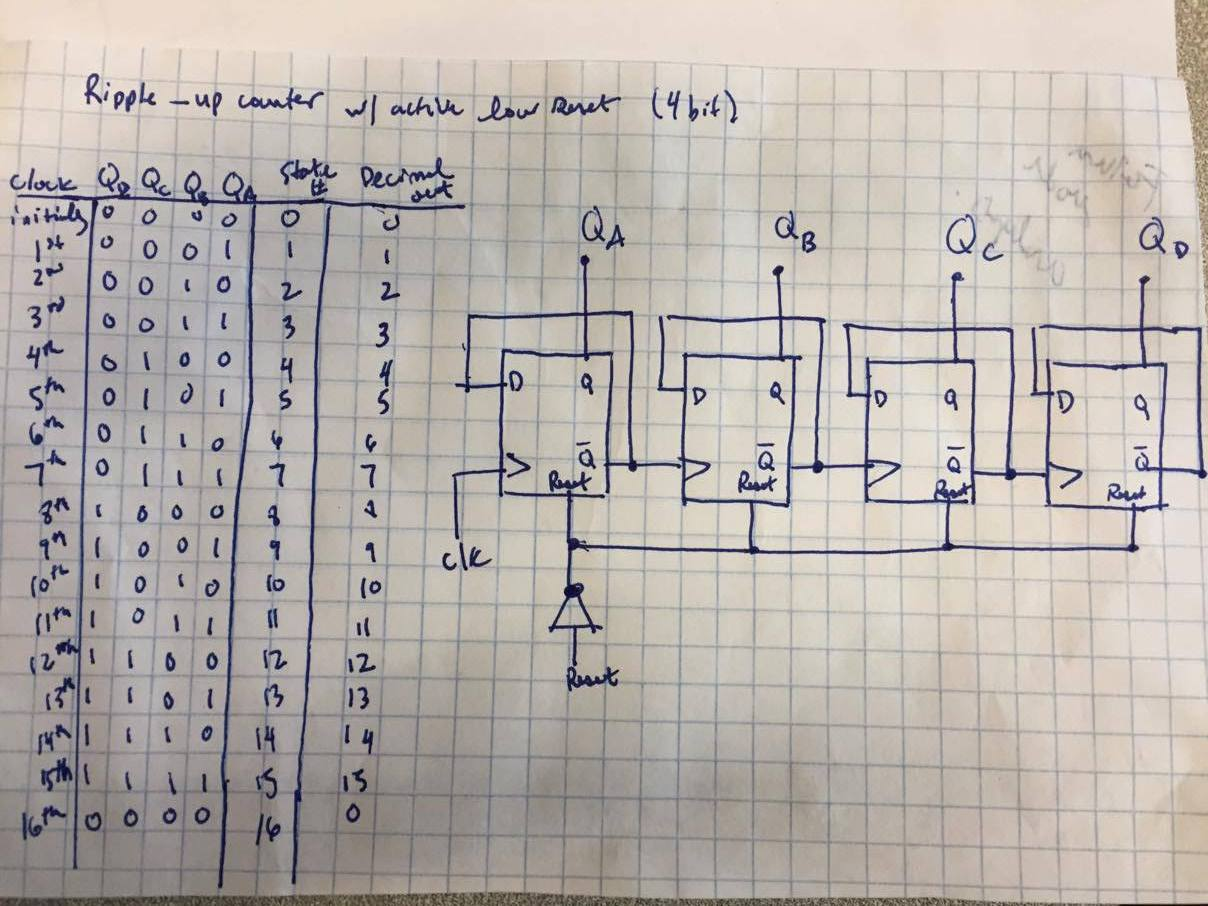
\includegraphics[width=0.5\linewidth]{figures/gate_diagrams/rippleUp_gate.jpg}
			\caption{Ripple-up counter logic reduction}
		\end{figure}

		\begin{figure}[H]
			\centering
			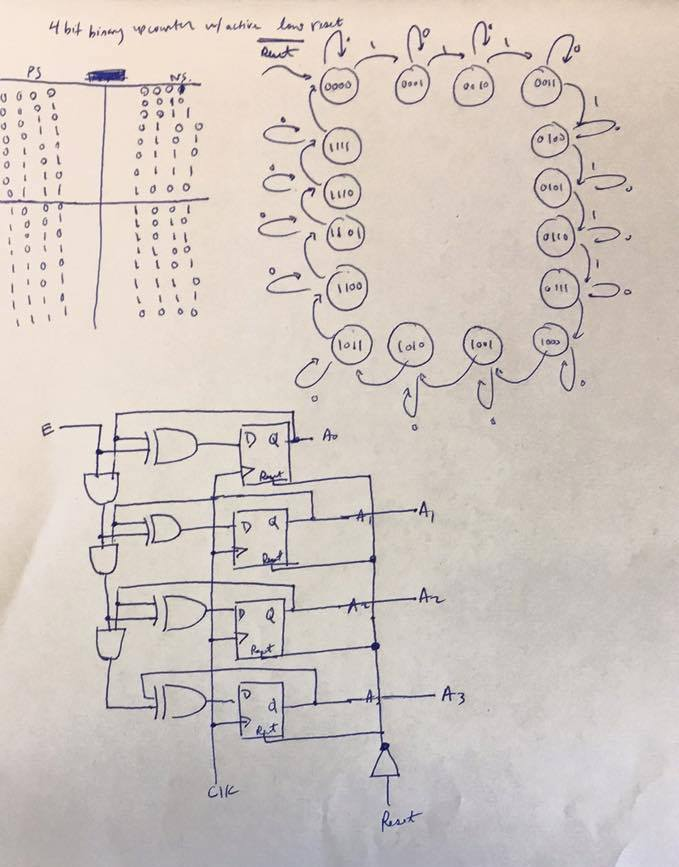
\includegraphics[width=0.5\linewidth]{figures/gate_diagrams/synchUp_gate.jpg}
			\caption{Synchronous up counter logic reduction}
		\end{figure}

		\begin{figure}[H]
			\centering
			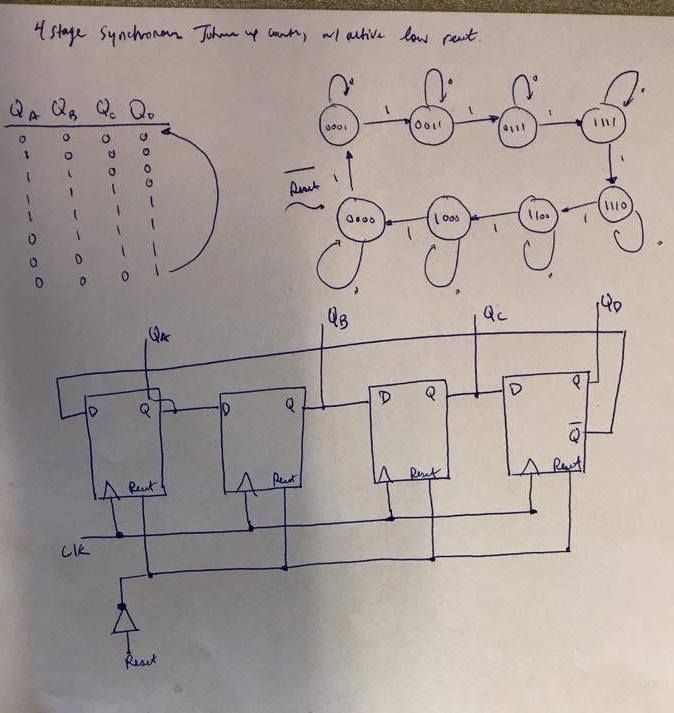
\includegraphics[width=0.5\linewidth]{figures/gate_diagrams/johnson_gate.jpg}
			\caption{Johnson counter logic reduction}
		\end{figure}


	\subsubsection{Verilog code}
		\paragraph{Ripple-up counter} The ripple-up counter, implemented at the gate-level
		\lstinputlisting[language=Verilog]{../counters/rippleUpCounter.sv}
		\lstinputlisting[language=Verilog]{../counters/rippleUpCounter_tester.v}

		\paragraph{Synchronous up counter} The synchronous up counter, implemented at the dataflow level
		\lstinputlisting[language=Verilog]{../counters/synUpCounter.sv}
		\lstinputlisting[language=Verilog]{../counters/synUpCounter_tester.v}

		\paragraph{Johnson Counter} The johnson counter, implemented at the behavioural level
		\lstinputlisting[language=Verilog]{../counters/johnsonCounter.sv}
		\lstinputlisting[language=Verilog]{../counters/johnsonUpCounter_tester.v}

		\paragraph{Synchronous up counter (schematic entry)} Schematic of the synchronous up counter, designed using Quartus' schematic entry

		\begin{figure}[H]
			\centering
			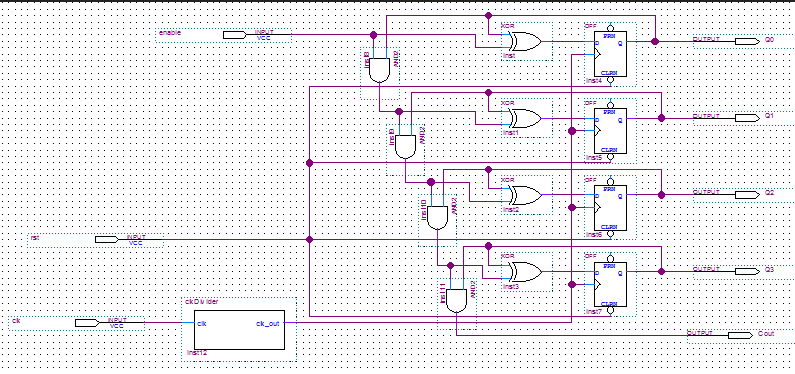
\includegraphics[width=0.75\linewidth]{figures/gate_diagrams/schem_synUp.png}
			\caption{Synchronous counter schematic entry}
			\label{fig:synUp_schem}
		\end{figure}

		\paragraph{} The generated verilog code \& tester
		\lstinputlisting[language=Verilog]{../counters/schem_synUp.v}
		\lstinputlisting[language=Verilog]{../counters/schem_synUp_tester.v}


	\subsubsection{RTL views}
		\begin{figure}[H]
		  \centering
		  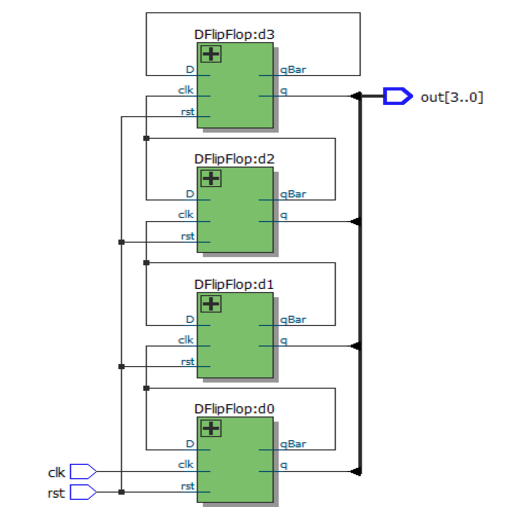
\includegraphics[width=0.75\linewidth]{figures/RTLs/rippleUp_RTL.png}
		  \caption{Ripple-up counter RTL view}
		  \label{fig:rippleUp_RTL}
		\end{figure}
		  
		\begin{figure}[H]
		  \centering
		  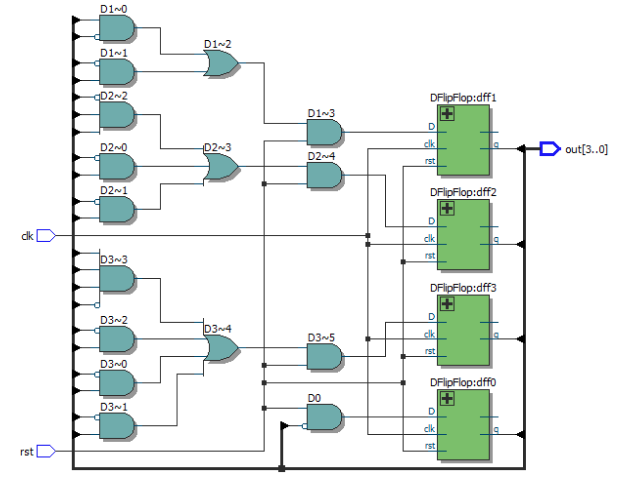
\includegraphics[width=0.75\linewidth]{figures/RTLs/synUp_RTL.png}
		  \caption{Synchronous up counter RTL view}
		  \label{fig:synUp_RTL}
		\end{figure}

		\begin{figure}[H]
		  \centering
		  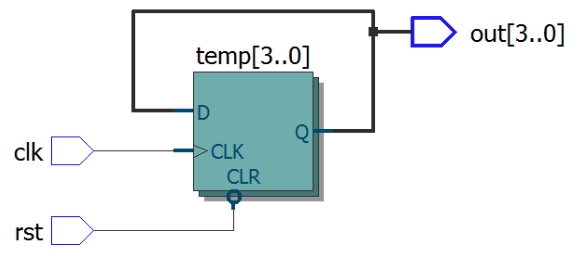
\includegraphics[width=0.75\linewidth]{figures/RTLs/johnson_RTL.png}
		  \caption{Johnson counter RTL view}
		  \label{fig:johnson_RTL}
		\end{figure}

		\begin{figure}[H]
		  \centering
		  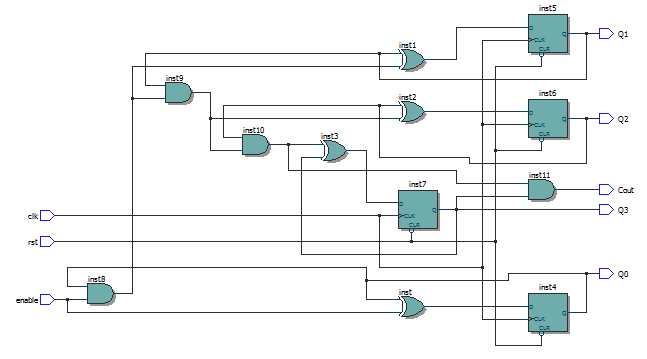
\includegraphics[width=0.75\linewidth]{figures/RTLs/schem_synUp_RTL.png}
		  \caption{Schematic entry synchronous counter RTL view}
		  \label{fig:schem_synUp_RTL}
		\end{figure}


	\subsubsection{Waveforms}
		\paragraph{} We simulated our designs using iverilog \& gtkwave

		\begin{figure}[H]
		  \centering
		  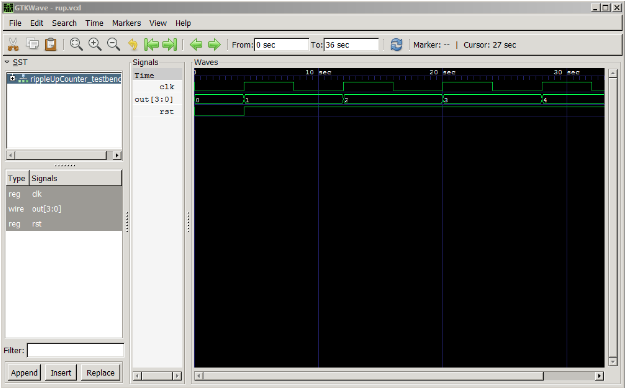
\includegraphics[width=0.75\linewidth]{figures/waveforms/rippleUp_wave.png}
		  \caption{Ripple-up counter waveform in gtkwave}
		  \label{fig:rippleUp_waveform}
		\end{figure}

		\begin{figure}[H]
		  \centering
		  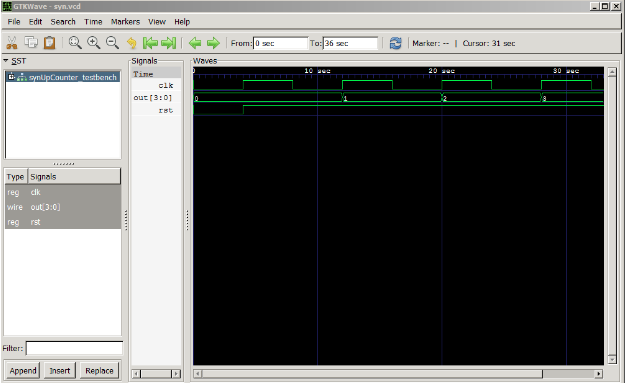
\includegraphics[width=0.75\linewidth]{figures/waveforms/synUp_wave.png}
		  \caption{Synchronous up counter waveform}
		  \label{fig:synUp_waveform}
		\end{figure}

		\begin{figure}[H]
		  \centering
		  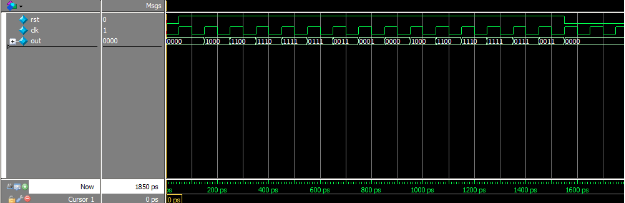
\includegraphics[width=0.75\linewidth]{figures/waveforms/johnson_wave.png}
		  \caption{Johnson counter waveform in gtkwave}
		  \label{fig:johnson_waveform}
		\end{figure}

		\begin{figure}[H]
		  \centering
		  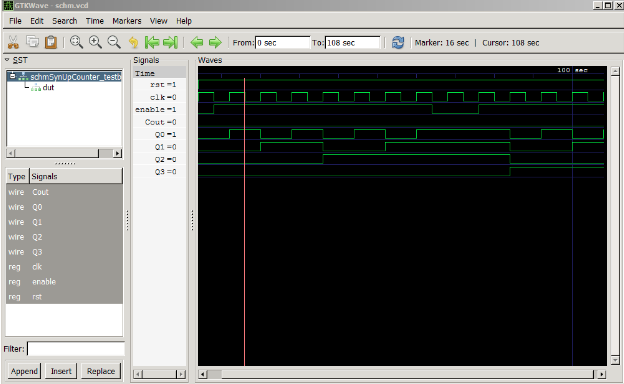
\includegraphics[width=0.75\linewidth]{figures/waveforms/schem_synUp_wave.png}
		  \caption{Synchronous up counter (schematic entry) waveform in gtkwave}
	   	  \label{fig:schem_synUp_waveform}
		\end{figure}


\subsection{Signal Tap II}
	\paragraph{} We checked our designs in real-time using Signal Tap II

	\paragraph{Ripple-up counter Signal Tap II waveform}
	\begin{figure}[H]
	  \centering
	  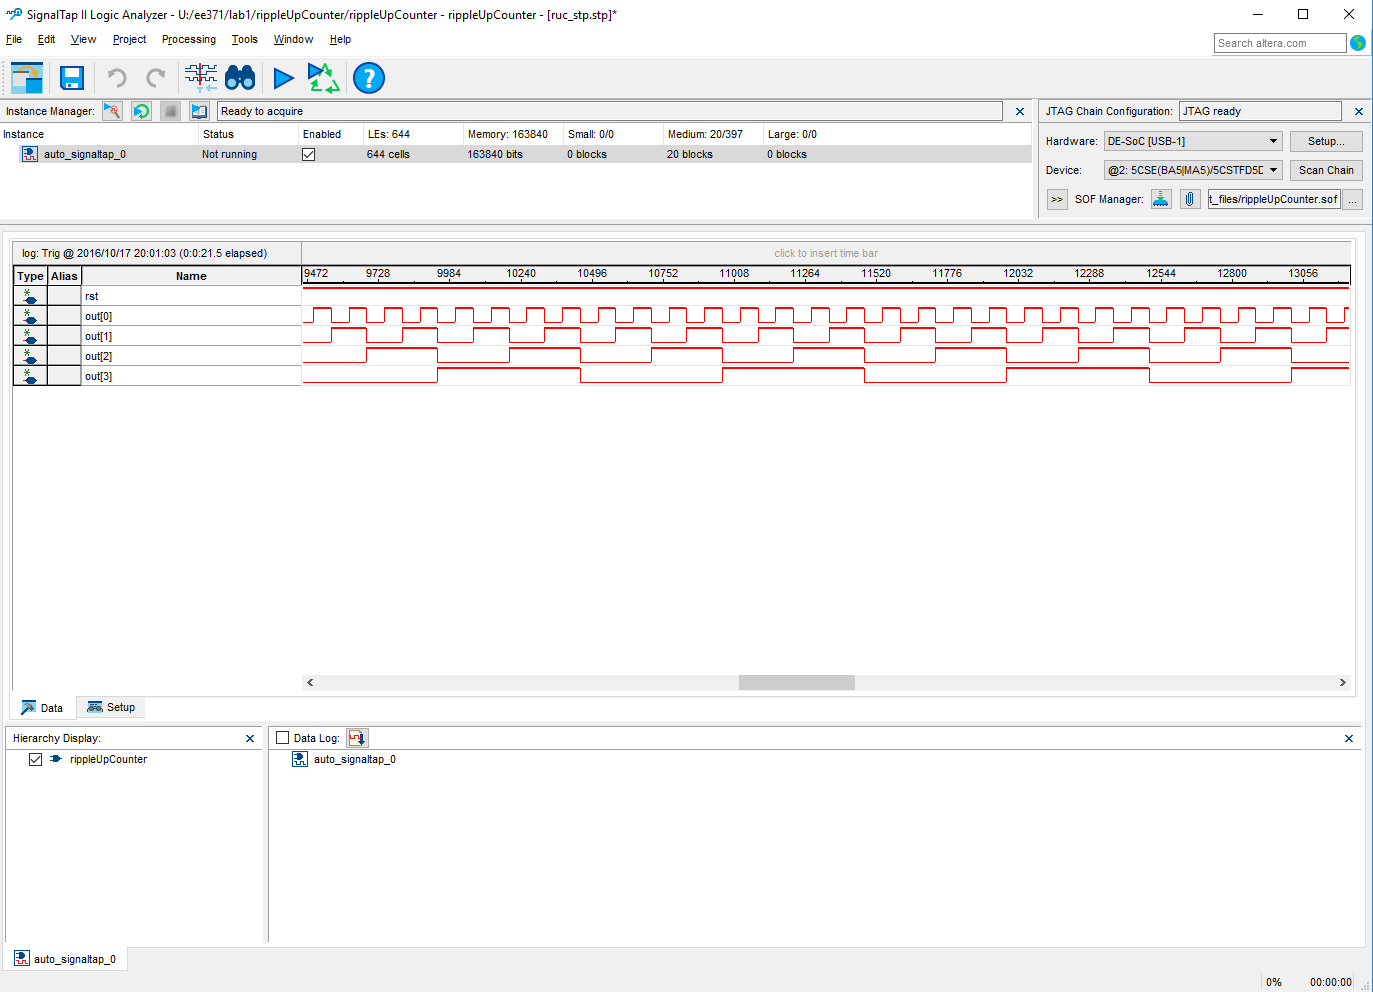
\includegraphics[width=0.75\linewidth]{figures/stp/rippleUp_stp.png}
	  \caption{Signal Tap II on ripple-up counter}
	  \label{fig:rippleUp_stp}
	\end{figure}

	\paragraph{Synchronous up counter Signal Tap II waveform}
	\begin{figure}[H]
	  \centering
	  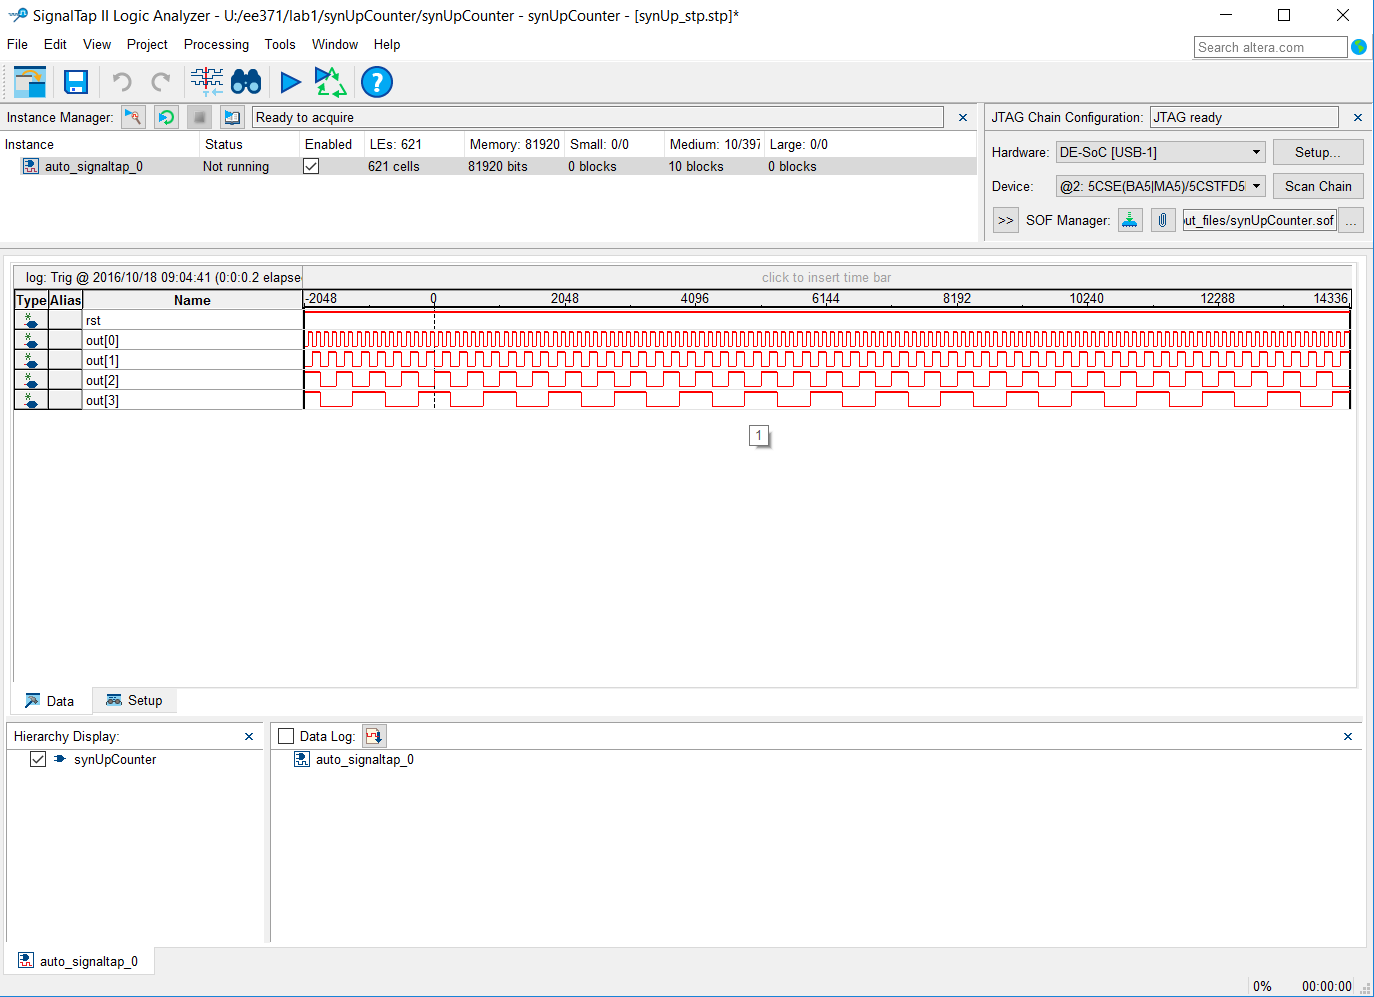
\includegraphics[width=0.75\linewidth]{figures/stp/synUp_stp.png}
	  \caption{Signal Tap II on synchronous up counter}
	  \label{fig:synUp_stp}
	\end{figure}

	\paragraph{Johnson counter Signal Tap II waveform}
	\begin{figure}[H]
	  \centering
	  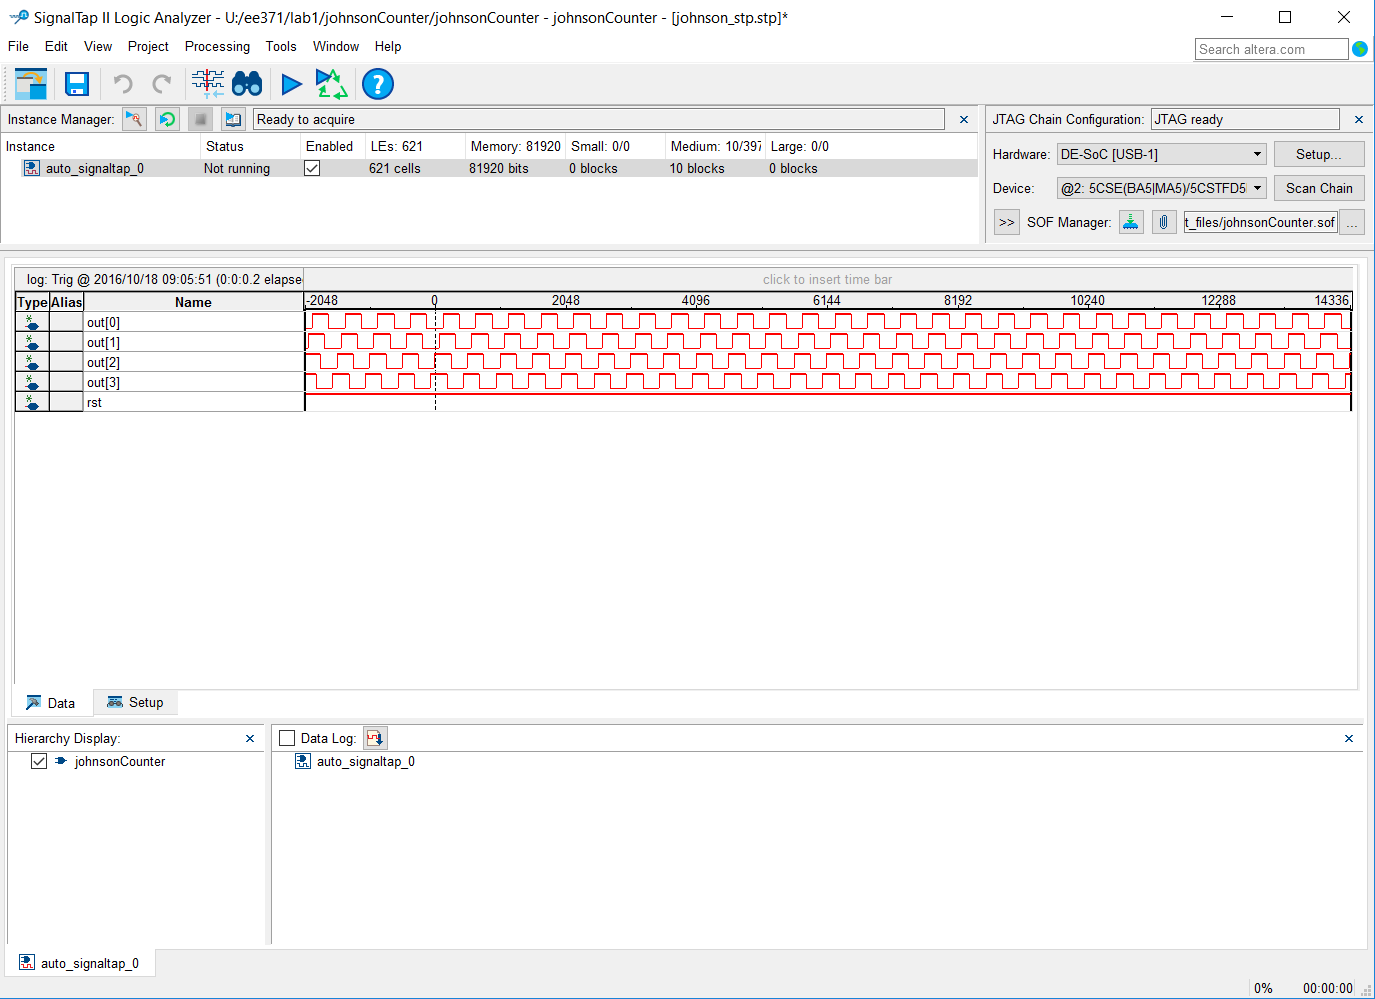
\includegraphics[width=0.75\linewidth]{figures/stp/johnson_stp.png}
	  \caption{Signal Tap II on johnson counter}
	  \label{fig:johnson_stp}
	\end{figure}

	\paragraph{Schematic entry synchronous up counter Signal Tap II waveform}
	\begin{figure}[H]
	  \centering
	  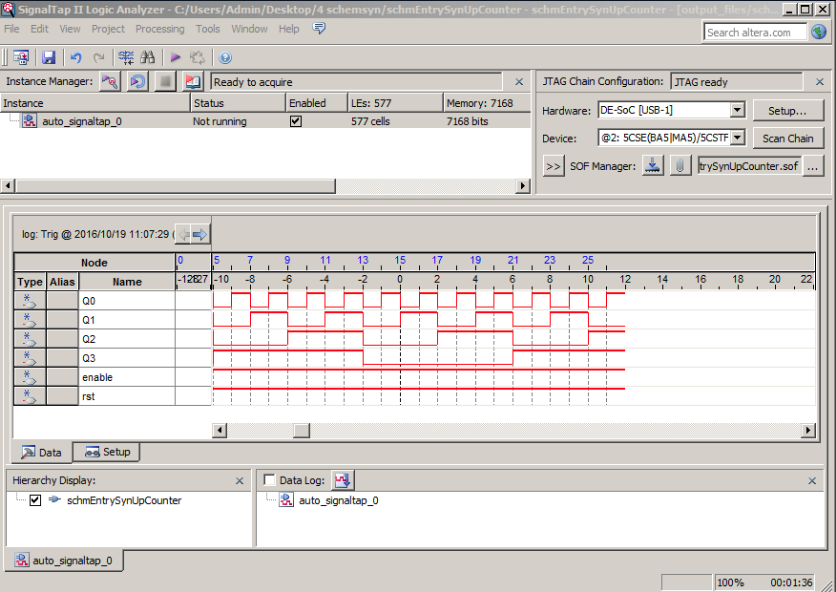
\includegraphics[width=0.75\linewidth]{figures/stp/schem_synUp_stp.png}
	  \caption{Signal Tap II on schematic entry synchronous up counter}
	  \label{fig:schem_synUp_stp}
	\end{figure}


\subsection{iverilog \& gtkwave}
	\paragraph{} We were provided verilog code to test, as an introduction to iverilog and gtkwave.

	\lstinputlisting[language=Verilog]{../iverilog_gtkwave/andOr0.v}
	\lstinputlisting[language=Verilog]{../iverilog_gtkwave/andorTop0.v}
	\lstinputlisting[language=Verilog]{../iverilog_gtkwave/testBench.v}

	\begin{figure}[H]
	  \centering
	  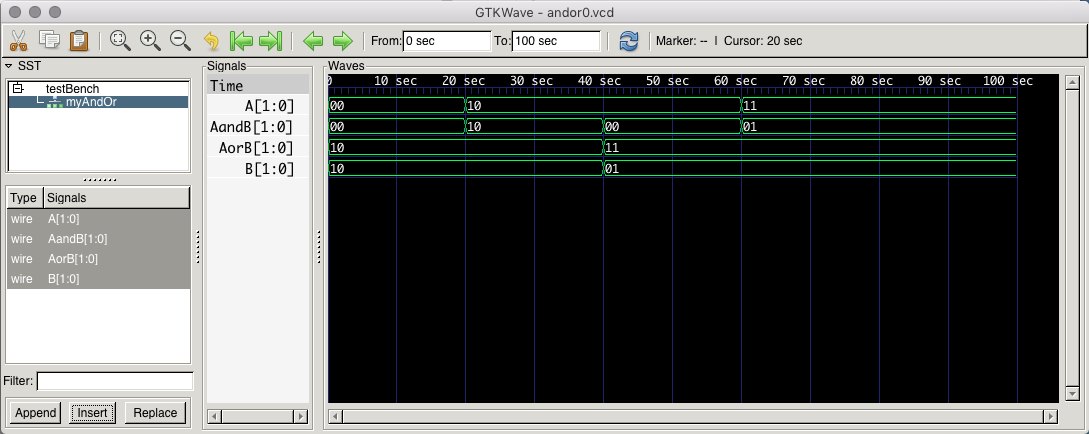
\includegraphics[width=0.75\linewidth]{figures/iverilog_gtkwave.png}
	  \caption{Results of iverilog \& gtkwave}
	  \label{fig:iverilog_gtkwave}
	\end{figure}


\subsection{Learning the C language}
	\paragraph{} The car listPrice C program we wrote, and the console output results
	\lstinputlisting[language=C]{../c_project/listPrice/listPrice.c}

	\begin{figure}[H]
		\centering
		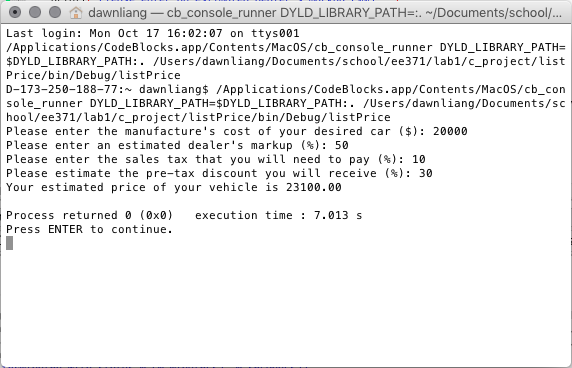
\includegraphics[width=0.75\linewidth]{figures/listPrice_results.png}
		\caption{listPrice program results}
		\label{fig:listPrice_results}
	\end{figure}

	\paragraph{} We were also required to write a detailed specification document for our car list price calculator.

	\subsubsection{Requirements Documentation}
		\paragraph{Abstract} The calculator program is a project that calculates the user’s desired car price given four estimated criteria: manufacture’s cost, dealer markup price, sales tax, and pretax discount. The estimated information is then taken in, and processed using a simple equation.  Our program results had matched up to our expectations, outputting the correct value given the four estimated costs as input.

		\paragraph{Introduction} This project gave us an overview to the basics of C programming and the CodeBlocks IDE. The result of this project was a program that allows the user to be able to estimate his/her car price based on a few estimated values. 

		\paragraph{Inputs}
		\begin{enumerate}
			\item The manufacture’s cost of the vehicle chosen by the user. This input is used to help give the initial base price to what the user is expected to pay.
			\item The estimated dealer’s markup price chosen by the user. This input is used to help give the user an idea of how much more he/she needs to pay in addition to the base price.
			\item The estimated sales tax chosen by the user. This input is used to figure out the additional costs associated from tax levied by the government on the vehicle.
			\item The dealer discount chosen by the user. This input is used to help reduce the total price (before tax) of the car the user will pay.
		\end{enumerate}

		\paragraph{Outputs} The program will output the total price of the vehicle after the user inputs the manufacturing costs, estimated dealer markup, the sales tax, and the dealer discount. 

		\paragraph{Major Functions} This program gives the user an estimation of the total price of the vehicle based on four estimated input cost values. The estimated input values are manufacturing costs, estimated dealer markup, sales tax and the dealer discount. 


	\subsubsection{Design Specification}
		\paragraph{Abstract} The listPrice program is a project that calculates the user’s desired car price given four estimated criteria: manufacture’s cost, dealer markup price, sales tax, and pretax discount. The estimated information was then taken in, and processed using a simple equation. Written in C and the CodeBlocks IDE, listPrice is our first program that provides taught us the fundamental basics of how to program in C. Our program results have matched up to our expectations, outputting the correct value given the four estimated costs as input.

		\paragraph{Introduction} This project gave us an overview to the basics of C programming and the CodeBlocks IDE. The result of this project was a program that allows the user to be able to estimate his/her car price based on a few estimated values. 

		\paragraph{Inputs} All values entered into listPrice must be entered as doubles. If any other value is entered (for instance, a string or a character), then the program will fail and not output the correct calculated answer. 
		\begin{enumerate}
			\item Manufacture’s cost of the vehicle: must be a positive number, and cannot be 0. If it is less than 0, then the output of the total car price will be negative.
			\item Estimated dealer markup: must be greater than or equal to 0, and entered as a percentage between 0 and 100 (for instance 5\% markup is entered as a 5). If the markup is less than 0, then the dealer will be losing money. 
			\item Estimated Sales Tax: must be greater than or equal to 0, and entered as a percentage that is greater than 0 (for instance 9.7\% sales tax is entered in as 9.7). If the tax is less than 0, then the user will receive an unintentional discount from the government.
			\item Dealer Discount: must be greater or equal to 0, and entered as a percentage between 0 and 100 (for instance a 2\% discount is entered as a 2). If the discount is less than 0, then the final price of the vehicle will be greater than if no discount had been applied. If the dealer discount is greater than 100, then the resulting vehicle price will be negative.
		\end{enumerate}

		\paragraph{Outputs} Outputs the total calculated cost of the vehicle as a double. The output is expected to be greater than 0. If the output is negative, then one or more of the inputs were incorrectly inputted into the program. 

		\paragraph{Major Functions} The listPrice program calculates the total cost of the vehicle given four estimated price inputs. Each input is taken in as a double, and then computed using the formula: 
		\[list\_price = in\_price \times (1 + \frac{markup\_price}{100}) \times (1 - \frac{discount\_price}{100}) \times (1 + \frac{tax\_percentage}{100})\]
		The output of the vehicle cost is the total cost that the user should expect to the pay if he/she were to purchase that particular vehicle.

\end{document}